\usetikzlibrary{decorations.markings}
\newcommand{\bigO}{\mathcal{O}}

\subsection{Integration of Complex Functions}
\subsubsection{Path Integrals}
Given that complex functions exist in a two-dimensional space, it is natural to consider integration over a path in the complex plane.\\
We can come up with a parameterization to express this path as a function of a real variable $t$:
\[w(t) = x(t) + iy(t)\]
\[\int_a^b w(t)dt=\int_a^b x(t)dt+i\int_a^b y(t)dt\]
Complex integrals will have the same properties as real integrals, such as linearity. One new property for complex integrals is:
\[\brvertical{\int_a^bw(t)dt}\leq\brvertical{\int_a^b|w(t)|dt}\]
\begin{proof}
\begin{align*}
    &\int_a^b w(t)dt=\rho e^{i\varphi}\\
    &\rho =\brvertical{\int_a^bw(t)dt}\\
    &\rho=e^{-i\varphi}\int_a^bw(t)dt=\int_a^bw(t)e^{-i\varphi}dt\\
    &\rho=\brvertical{\int_a^bw(t)dt}=\int_a^be^{-it}w(t)dt=\Re\brround{\int_a^be^{-i\varphi}w(t)dt}\\
    &\rho=\int_a^b\Re\brround{e^{-i\varphi}w(t)}dt\leq\int_a^b\brvertical{e^{-i\varphi}w(t)}dt=\int_a^b|w(t)|dt
\end{align*}
\end{proof}
A path or contour $C$ is a piecewise smooth curve in the complex plane.
\[C=z(t)=x(t)+iy(t),\ a\leq t\leq b\]
A path also has a direction, which is the direction of increasing $t$.
\[\int_C f(z)dz=\int_a^b f(z(t))z'(t)dt\]
\[dz=z'(t)dt=(x'(t)+iy'(t))dt\]
Ex: $f(x,y)=x-2xyi$
\begin{align*}
    &\int_C (x-2xyi)dz,\ C=\brcurly{y=x^2,0\leq x\leq 1}\cup\brcurly{y=1,-1\leq x\leq1}\\
    &f_1=x-2x^3i\\
    &z=x+iy=x+ix^2\Ra dz=(1+2xi)dx\\
    &\int_0^1(x-2x^3i)(1+2xi)dx=\int_0^1(x+2x^2i-2x^3i+4x^4)dx=\frac{1}{2}+\frac{2}{3}i-\frac{2}{4}i+\frac{4}{5}\\
    &f_2=x-2xi\\
    &z=x+iy=x+i\Ra dz=dx\\
    &\int_{-1}^1(x-2xi)dx=\brsquare{\frac{x^2}{2}-x^2i}_{-1}^1=0\\
    &\int_C (x-2xyi)dz=\frac{13}{10}+\frac{1}{6}i
\end{align*}
A closed path (has the same start and end points) is called a contour. It is the same as a path integral but we will see later that contours have special properties with complex functions.\\
Ex2: $f(z)=\bar{z}^2$ on the contour $C$ that is the box with vertices $0,1,1+i,i,0$ in the counterclockwise direction.
\begin{align*}
    &\overline{z}^2=(x-iy)^2=x^2-2xyi-y^2\\
    &y=0:\ f_1=x^2\\
    &z=x+iy=x\Ra dz=dx\\
    &\int_{C_1}f_1dz=\int_0^1 x^2dx=\frac{1}{3}\\
    &x=1:\ f_2=1-2yi-y^2\\
    &z=x+iy=1+iy\Ra dz=idy\\
    &\int_{C_2}f_2dz=\int_0^1(1-2yi-y^2)idy=\brsquare{iy+y^2-\frac{y^3}{3}i}_0^1=i+1-\frac{i}{3}=\frac{2}{3}i+1\\
    &y=1:\ f_3=x^2-2xi-1\\
    &z=x+iy=x+i\Ra dz=dx\\
    &\int_{C_3}f_3dz=-\int_0^1(x^2-2xi-1)dx=-\frac{1}{3}+i+1=i+\frac{2}{3}\\
    &x=0:\ f_4=-y^2\\
    &z=x+iy=iy\Ra dz=idy\\
    &\int_{C_4}f_4dz=-\int_0^1(-y^2)idy=\frac{i}{3}\\
    &\int_C\overline{z}^2dz=2+2i
\end{align*}
Ex3: $f(z)=\Log(z)$
\begin{align*}
    &C=\brcurly{|z|=1,\Re(z)\geq0}\\
    &z=e^{it},\ -\frac{\pi}{2}\leq t\leq \frac{\pi}{2}\\
    &dz=ie^{it}dt\\
    &\int_C\Log(z)dz=\int_{-\frac{\pi}{2}}^{\frac{\pi}{2}}\Log(e^{it})\brround{ie^{it}}dt=-\int_{-\frac{\pi}{2}}^{\frac{\pi}{2}}te^{it}dt\\
    &=-\frac{te^{it}}{i}\eval_{-\frac{\pi}{2}}^{\frac{\pi}{2}}+\int_{-\frac{\pi}{2}}^{\frac{\pi}{2}}\frac{e^{it}}{i}dt=-e^{it}\eval_{-\frac{\pi}{2}}^{\frac{\pi}{2}}=-2i
\end{align*}
\subsubsection{Fundamental Theorem of Calculus}
A neat property of complex integrals is that they are path independent. This means that the value of the integral is the same for any path between the start and end points. This is not true for real integrals.\\
Ex: Given the function $f(z)=z^2+1$ we will compute three different integrals between the points $z_1=-i$ and $z_2=1$ and show that they are all equal.\\
Path 1:
\begin{align*}
    &C=\brcurly{y=x-1}\\
    &z^2+1=(x+iy)^2+1=x^2+2xyi-y^2+1\\
    &\int_C(x^2-y^2+1+2xyi)dz\\
    &z=x+iy=x+i(x-1)\Ra dz=(1+i)dx\\
    &\int_0^1(x^2-(x-1)^2+1+2x(x-1)i)(1+i)dx\\
    &=\int_0^1(2x+2x^2i-2xi)(1+i)dx=\brsquare{x^2+\frac{2x^3}{3}i-x^2i}_0^1(1+i)\\
    &=\brround{1-\frac{i}{3}}(1+i)=\frac{4}{3}+\frac{2}{3}i
\end{align*}
Path 2:
\begin{align*}
    &C=\brcurly{x=0,-1\leq y\leq 0}\cup\brcurly{y=0,0\leq x\leq 1}\\
    &C_1:\ \int_{-1}^0(-y^2+1)idy=\brsquare{y-\frac{y^3}{3}}_{-1}^0i=\frac{2}{3}i\\
    &C_2:\ \int_0^1(x^2+1)dx=\brsquare{\frac{x^3}{3}+x}_0^1=\frac{4}{3}\\
    &\int_C(z^2+1)dz=\frac{4}{3}+\frac{2}{3}i
\end{align*}
Path 3:
\begin{align*}
    &z=e^{it},\ -\frac{\pi}{2}\leq t\leq 0\\
    &z^2+1=e^{2it}+1\\
    &dz=ie^{it}dt\\
    &\int_{-\frac{\pi}{2}}^0\brround{e^{2it}+1}ie^{it}dt=i\int_{-\frac{\pi}{2}}^0\brround{e^{3it}+e^{it}}dt=i\brsquare{\frac{e^{3it}}{3i}+\frac{e^{it}}{i}}_{-\frac{\pi}{2}}^0=\frac{4}{3}-\frac{e^{-i\frac{3\pi}{2}}}{3}-e^{-i\frac{\pi}{2}}\\
    &=\frac{4}{3}+\frac{2}{3}i
\end{align*}
This finding leads us to the Fundamental Theorem of Calculus for complex integrals.
$$\int_C f(z)dz=F(z_2)-F(z_1)$$
where $F'(z)=f(z)$.\\
When an antiderivative of $f(z)$ exits it becomes far easier to compute the integral.\\
Ex:
\begin{align*}
    &\int_C\sin zdz,\ C:\ e^{it},\ -\frac{\pi}{2}\leq t\leq \frac{5\pi}{4}\\
    &\int_C\sin z dz= -\cos z_1+\cos z_0\\
    &z_0=e^{-i\frac{\pi}{2}}=-i\\
    &z_1=e^{i\frac{5\pi}{4}}=-\frac{1}{\sqrt{2}}-\frac{1}{\sqrt{2}}i\\
    &\cos(z)=\cos(x)\cosh(y)-i\sin(x)\sinh(y)\\
    &\cos(z_0)=\cosh(1)\\
    &\cos(z_1)=\cos\bfrac{1}{\sqrt{2}}\cosh\bfrac{1}{\sqrt{2}}-i\sin\bfrac{1}{\sqrt{2}}\sinh\bfrac{1}{\sqrt{2}}\\
    &\int_C\sin zdz=\cos(-i)-\cos\brround{-\frac{1}{\sqrt{2}-\frac{1}{\sqrt{2}}i}}=\cosh(1)-\cos\bfrac{1}{\sqrt{2}}\cosh\bfrac{1}{\sqrt{2}}+i\sin\bfrac{1}{\sqrt{2}}\sinh\bfrac{1}{\sqrt{2}}
\end{align*}
Ex2:
\begin{align*}
    &\int_C\frac{dz}{z},\ C:\ \frac{x^2}{4}+y^2=1,\ y\geq0\\
    &\int_C\frac{dz}{z}=\log^*(z)=\ln|z|+i\varphi\eval_{z_0}^{z_1},\ \varphi\in\brround{-\frac{\pi}{2},\frac{3\pi}{2}}\\
    &y=0:\ \frac{x^2}{4}=1\Ra x=\pm2\\
    &z_0=2,\ z_1=-2\\
    &\int_C\frac{dz}{z}=\ln2+\pi i-\ln2=\pi i
\end{align*}
Ex3:
\begin{align*}
    &\int_C\frac{dz}{z^2},\ C:\ \frac{x^2}{4}+y^2=1,\ y\geq0\\
    &\int_C\frac{dz}{z^2}=-\frac{1}{z_1}+\frac{1}{z_0}\\
    &z_0=2,\ z_1=-2\\
    &\int_C\frac{dz}{z^2}=\frac{1}{2}+\frac{1}{2}=1
\end{align*}
Ex4:
\begin{align*}
    &\int_C\frac{dz}{z},\ C:\ z=e^{it},\ 0\leq t\leq \frac{3\pi}{2}\\
    &\int_C\frac{dz}{z}=\ln|z|+i\varphi\eval_{z_0}^{z_1},\ \varphi\in\brround{-\frac{\pi}{4},\frac{7\pi}{4}}\\
    &z_0=e^{0}=1\\
    &z_1=e^{i\frac{3\pi}{2}}=-i\\
    &\int_C\frac{dz}{z}=\brround{\ln(1)+\frac{3\pi}{2}i}-\brround{\ln(1)+0}=\frac{3\pi}{2}i
\end{align*}
Ex5:
\begin{align*}
    &\int_C z^{1/3}dz,\ C:\ r=2\cos\bfrac{\theta}{2},\ -\frac{\pi}{2}\leq\theta\leq\frac{\pi}{2}\\
    &\int_Cz^{1/3}dz=\frac{3}{4}z^{4/3}\eval_{z_0}^{z_1}=\frac{3}{4}|z|^{4/3}e^{i\varphi}\eval_{z_0}^{z_1},\ \varphi\in\brround{-\pi,\pi}\\
    &r\brround{\pm\frac{\pi}{2}}=2\cos\bfrac{\pi}{4}=\frac{2}{\sqrt{2}}=\sqrt{2}\\
    &z_0=-\sqrt{2}i,\ z_1=\sqrt{2}i\\
    &\int_C z^{1/3}dz=\frac{3}{4}(\sqrt{2})^{4/3}\brround{e^{i\frac{2\pi}{3}}-e^{-i\frac{2\pi}{3}}}\\
    &\int_C z^{1/3}dz=\frac{3}{2^{1/3}}\frac{i}{2i}\brround{e^{i\frac{2\pi}{3}}-e^{-i\frac{2\pi}{3}}}=\frac{3i}{2^{1/3}}\sin\bfrac{2\pi}{3}
\end{align*}
Ex6:
\begin{align*}
    &\int_C\Log(z)dz,\ C:\ r=2\cos\bfrac{\theta}{2},\ -\frac{\pi}{2}\leq\theta\leq\frac{\pi}{2}\\
    &z_0=-\sqrt{2}i,\ z_1=\sqrt{2}i\\
    &\int_C\Log zdz=\brsquare{z\Log z-z}_{-\sqrt{2}i}^{\sqrt{2}i}=\sqrt{2}i\brround{\ln\sqrt{2}+i\frac{\pi}{2}-1}+\sqrt{2}i\brround{\ln\sqrt{2}-i\frac{\pi}{2}-1}\\
    &=\brround{2\sqrt{2}\ln\sqrt{2}-2\sqrt{2}}i
\end{align*}
Another property of complex integrals we will make use of often is the inequality
\[\brvertical{\int_C f(z)dz}\leq \max_{z\in C}|f(z)|\cdot\text{Length}(C)\]
\begin{proof}
\begin{align*}
    \brvertical{\int_C f(z)dz}&=\brvertical{\int_a^b f(z(t))z'(t)dt}\\
    &\leq\brvertical{\int_a^b |f(z(t))||z'(t)|dt}\\
    &\leq\max_{a\leq t\leq b}|f(z(t))|\cdot\int_a^b\sqrt{x^2+y^2}dt\\
    &\leq\max_{z\in C}|f(z)|\cdot\text{Length}(C)
\end{align*}
\end{proof}
Ex: Prove the inequality
\[
\brvertical{\int_C\frac{dz}{z^2+i}}\leq\frac{3\pi}{4}
\]
$C$ is the circle $|z|=3$ traversed once
\begin{proof}
    \begin{align*}
        &\brvertical{\int_Cf(z)dz}\leq\max_{z\in C}|f(z)|\mathrm{Length}(C)\\
        &\mathrm{Length}(C)=6\pi\\
        &\brvertical{\int_C\frac{dz}{z^2+i}}\leq6\pi\max_{z\in C}\brvertical{\frac{1}{z^2+i}}\\
        &\max_{z\in C}\brvertical{\frac{1}{z^2+i}}=\frac{1}{\min\limits_{z\in C}|z^2+i|}\\
        &|z^2+i|\geq\brvertical{|z^2|-|i|}=|9-1|=8\\
        &\min_{z\in C}|z^2+i|=8\\
        &\max_{z\in C}\brvertical{\frac{1}{z^2+i}}=\frac{1}{8}\\
        &\brvertical{\int_C\frac{dz}{z^2+i}}\leq\frac{6\pi}{8}=\frac{3\pi}{4}
    \end{align*}
\end{proof}
Ex2: Prove the inequality
\[
\brvertical{\int_C\Log(z)dz}\leq\frac{\pi^2}{2}
\]
where $C$ is described by $e^{it},\ -\frac{\pi}{2}\leq t\leq\frac{\pi}{2}$
\begin{proof}
Note that the curve is a semicircle of radius 1 where $x\geq0$.
\begin{align*}
    &\brvertical{\int_Cf(z)dz}\leq\max_{z\in C}|f(z)|\mathrm{Length}(C)\\
    &\mathrm{Length}(C)=\pi\\
    &f(z)=\Log z=\ln|z|+i\varphi,\ \varphi\in\brround{-\pi,\pi}\\
    &\max_{z\in C}|f(z)|=\max_{z\in C}|\Log z|=\max_{z\in C}|\ln|z|+i\varphi|\\
    &z=e^{it}\\
    &|z|=1\\
    &\varphi=t\\
    &\max_{z\in C}|f(z)|=\max_{-\frac{\pi}{2}\leq t\leq\frac{\pi}{2}}|it|=\max_{-\frac{\pi}{2}\leq t\leq\frac{\pi}{2}}|t|=\frac{\pi}{2}\\
    &\brvertical{\int_C\Log(z)dz}\leq\frac{\pi}{2}\cdot \pi=\frac{\pi^2}{2}
\end{align*}
\end{proof}
Ex3: Prove the inequality
\[
\brvertical{\int_C\frac{e^{3z}}{e^z+1}dz}\leq\frac{2\pi e^{3R}}{e^R-1}
\]
where $C$ is the vertical line segment from $z=R$ to $z=R+2\pi i$ such that $R\in\R$ and $R>0$.
\begin{proof}
\begin{align*}
    &\brvertical{\int_Cf(z)dz}\leq\max_{z\in C}|f(z)|\mathrm{Length}(C)\\
    &\mathrm{Length}(C)=2\pi\\
    &f(z)=\frac{e^{3z}}{e^z+1}
\end{align*}
Let us describe $C$ by
\begin{align*}
    &C:\ z=R+it,\ 0\leq t\leq 2\pi\\
    &\max_{z\in C}|f(z)|=\max_{z\in C}\brvertical{\frac{e^{3z}}{e^z+1}}=\max_{0\leq t\leq 2\pi}\brvertical{\frac{e^{3R}e^{3it}}{e^Re^{it}+1}}=\max_{0\leq t\leq 2\pi}\frac{e^{3R}}{|e^Re^{it}+1|}\\
    &\max_{0\leq t\leq 2\pi}\frac{1}{|e^Re^{it}+1|}=\frac{1}{\min\limits_{0\leq t\leq 2\pi}|e^Re^{it}+1|}\\
    &\min_{0\leq t\leq 2\pi}|e^Re^{it}+1|=\min_{0\leq t\leq 2\pi}|e^R\brround{\cos(t)+i\sin(t)}+1|=\min_{0\leq t\leq 2\pi}\sqrt{(e^R\cos(t)+1)^2+e^{2R}\sin^2(t)}\\
    &=\min_{0\leq t\leq 2\pi}\sqrt{e^{2R}\cos^2t+e^{2R}\sin^2t+2e^R\cos t+1}=\min_{0\leq t\leq 2\pi}\sqrt{e^{2R}+2e^R\cos t+1}\\
    &\min_{0\leq t\leq 2\pi}\cos t=-1\\
    &\min_{0\leq t\leq 2\pi}|e^Re^{it}+1|=\sqrt{e^{2R}-2e^R+1}=\sqrt{(e^R-1)^2}=|e^R-1|\\
    &R>0\Ra e^R>1\Ra |e^R-1|=e^R-1\\
    &\max_{z\in C}\brvertical{\frac{e^{3z}}{e^z+1}}=\frac{e^{3R}}{e^R-1}\\
    &\brvertical{\int_C \frac{e^{3z}}{e^z+1}dz}\leq\frac{2\pi e^{3R}}{e^R-1}
\end{align*}
\end{proof}

\subsubsection{Loop Integrals}
A loop, $C$, is a path such that $z_2=z_1$ (the start and end points are the same).\\
A simple closed loop is a loop with no other intersections. For example, a figure 8 is not a simple closed loop.\\
Using the FTC (Fundamental Theorem of Calculus) we can see that if $f(z)$ is continuous and has an antiderivative $F(z)$ in $\mathcal{D}$ then
\[\int_C f(z)dz=0\]
for any loops in $\mathcal{D}$.\\
Ex:
\begin{align*}
    &f(z)=\frac{\cos z}{z^2+6z+10}\\
    &z=\frac{-6\pm\sqrt{36-40}}{2}=-3\pm i
\end{align*}
$f(z)$ is analytic on $|z|\leq 2$
\[
\therefore\ \int_{|z|=2}f(z)dz=0
\]
Ex2:
\begin{align*}
    &f(z)=\Log(2z+5)\\
    &w=2z+5\\
    &\text{not analytic where }\Re(w)<0,\ \Im(w)=0\\
    &w=2x+5+iy\\
    &y=0\\
    &2x+5<0\Ra x<-\frac{5}{2}
\end{align*}
$f(z)$ is analytic on $|z|\leq 2$
\[
\therefore\ \int_{|z|=2}f(z)dz=0
\]
Ex3:
\begin{align*}
    &f(z)=\arcsin\bfrac{z}{3}\\
    &w=\frac{z}{3}\\
    &\text{not analytic where }|\Re(w)|>1,\ \Im(w)=0\\
    &w=\frac{x}{3}+i\frac{y}{3}\\
    &y=0\\
    &\frac{|x|}{3}>1\Ra |x|>3
\end{align*}
$f(z)$ is analytic on $|z|\leq 2$
\[
\therefore\ \int_{|z|=2}f(z)dz=0
\]
Ex4:
\begin{align*}
    &f(z)=\tan\bfrac{z}{2}=\frac{\sin\bfrac{z}{2}}{\cos\bfrac{z}{2}}\\
    &\cos\bfrac{z}{2}= 0\\
    &\frac{z}{2}=\frac{\pi}{2}+n\pi,\ n\in\Z\\
    &z=\pi+2\pi n=\brcurly{\cdots,-\pi,\pi,\cdots}
\end{align*}
$f(z)$ is analytic on $|z|\leq 2$
\[
\therefore\ \int_{|z|=2}f(z)dz=0
\]
Let us look at the slightly more general case of
\[\int_C (z-z_0)^ndz\]
where $C$ is a simple closed loop and $z_0$ is a point inside $C$.\\
\begin{center}
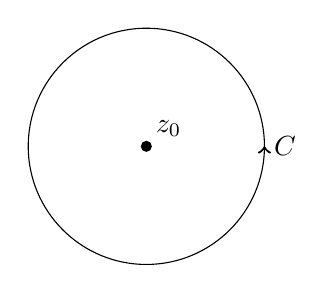
\begin{tikzpicture}
    % Point z_0
    \coordinate (z0) at (1.5,1);
    \fill (z0) circle (2pt);
    \node[above right] at (z0) {$z_0$};

    % Circle around z_0
    \draw (z0) circle (1.5);

    % Arrow pointing to z_0
    \draw[->, thick] (3,1);
    \node[right] at (3,1) {$C$};
\end{tikzpicture}
\end{center}
If $n\geq 0$,
\begin{align*}
    &\brround{\frac{1}{n+1}(z-z_0)^{n+1}}'=(z-z_0)^n\\
    &\Ra\int_C(z-z_0)^ndz=0
\end{align*}
If $n<0$ and $n\neq-1$,
\begin{align*}
    &\brround{\frac{1}{n+1}(z-z_0)^{n+1}}'=(z-z_0)^n\\
    &\Ra\int_C(z-z_0)^ndz=0
\end{align*}
If $n=-1$,
\begin{align*}
    &\int_C\frac{dz}{z-z_0}
\end{align*}
Let us assume that $z_0=0$ by shifting everything over by $z_0$.\\
$C=C_1\cup C_2$ where $C_1$ is the big loop from $z_1$ to $z_2$ and $C_2$ is the small line segment from $z_2$ to $z_1$.\\
\centerline{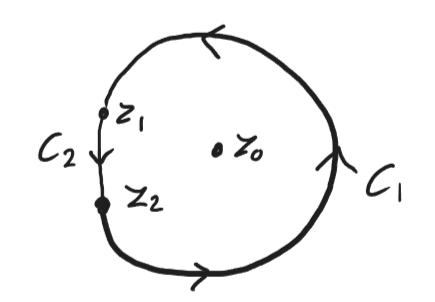
\includegraphics[width=0.3\textwidth]{Images/ComplexAnalysisPictures/LoopIntegralContinuity.png}}
\begin{align*}
    &\int_{C_1}\frac{dz}{z}=\Log(z_2)-\Log(z_1)\\
    &\brvertical{\int_{C_2}\frac{dz}{z}}\leq\max_{z\in C_2}\frac{1}{|z|}\cdot\text{Length}(C_2)\to0\text{ as $z_1=z_2$}\\
    &\Log z_2=\ln|z_2|+i\varphi_2\to \ln|z_0|+i\pi\\
    &\Log z_1=\ln|z_1|+i\varphi_1\to \ln|z_0|-i\pi\\
    &\int_C\frac{dz}{z}=\int_{C_1}\frac{dz}{z}+\int_{C_2}\frac{dz}{z}\to2 i\pi+0\\
    &\int_C\frac{dz}{z}=2\pi i
\end{align*}
And so we get
\[\int_C(z-z_0)^ndz=\eqnsystem{0 & \text{if $z_0$ is outside $C$}\\ 2\pi i & \text{if $z_0$ is inside $C$ and $n=-1$}\\ 0 & \text{if $z_0$ is inside $C$ and $n\neq-1$}}\]
This means that the result of a loop integral will only be nonzero if there is some singularity inside the loop.

\subsubsection{Deformation of Path}
Suppose $f(z)$ is analytic in $D$ then we can show
\[\int_C f(z)dz=\int_{C_0}f(z)dz\]
\centerline{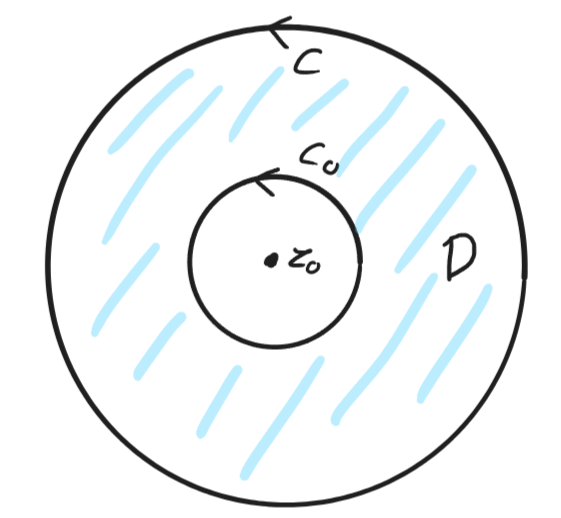
\includegraphics[width=0.4\textwidth]{Images/ComplexAnalysisPictures/DeformationOfPath.png}}
To show this, we will need a simply connected domain. We can construct the following contour:\\
\centerline{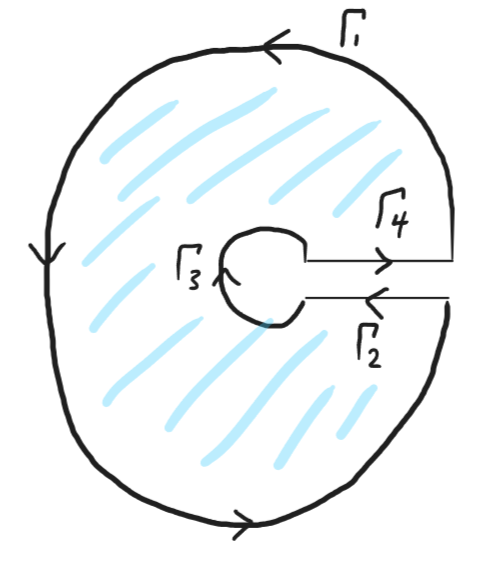
\includegraphics[width=0.3\textwidth]{Images/ComplexAnalysisPictures/SimplyConnectedDomain.png}}
We can define a new path, $C_\epsilon=\Gamma_1\cup\Gamma_2\cup\Gamma_3\cup\Gamma_4$.\\
Assuming that the function is well defined in the region $D$ then we get
\begin{align*}
    &\int_{C_\epsilon}f(z)dz=\int_{\Gamma_1}f(z)dz+\int_{\Gamma_2}f(z)dz+\int_{\Gamma_3}f(z)dz+\int_{\Gamma_4}f(z)dz=0
\end{align*}
In the limiting case we can see that
\begin{align*}
    &\int_{\Gamma_1}f(z)dz\to\int_{C}f(z)dz\\
    &\int_{\Gamma_3}f(z)dz\to-\int_{C_0}f(z)dz\\
    &\int_{\Gamma_2}f(z)dz+\int_{\Gamma_4}f(z)dz\to0
\end{align*}
And so we are left with
\begin{align*}
    &\int_{C_\epsilon}f(z)dz=\int_Cf(z)dz-\int_{C_0}f(z)dz=0\\
    &\Ra \int_Cf(z)dz=\int_{C_0}f(z)dz
\end{align*}
This means that any integral over a closed path is equal to the sum of closed path integrals around any singularities in the domain.\\
\centerline{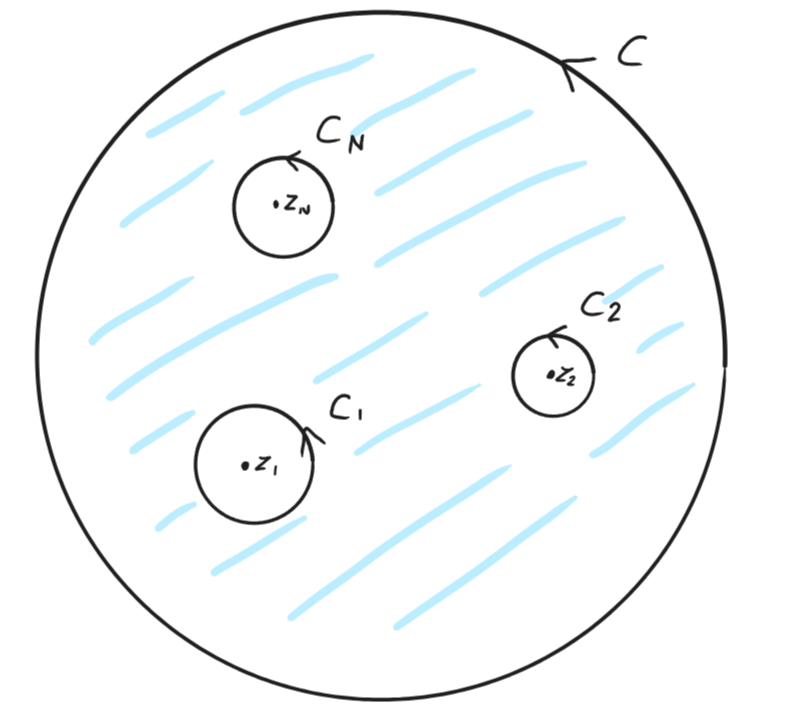
\includegraphics[width=0.6\textwidth]{Images/ComplexAnalysisPictures/MultipleSingularities.png}}
\[\int_Cf(z)dz=\sum_{j=1}^N\int_{C_j}f(z)dz\]
Ex:
\begin{align*}
    &\int_{|z|=2}\frac{dz}{z(z-1)}\\
    &C_1:\ |z-0|=r\\
    &C_2:\ |z-1|=r,\ \text{$r$ is small}\\
    &I=\int_{|z|=2}f(z)dz=\int_{|z-0|=r}\frac{dz}{z(z-1)}+\int_{|z-1|=r}\frac{dz}{z(z-1)}\\
    &\frac{1}{z(z-1)}=\frac{A}{z}+\frac{B}{z-1}=\frac{A(z-1)+Bz}{z(z-1)}=\frac{(A+B)z-A}{z(z-1)}\\
    &\eqnsystem{A+B=0\\ -A=1}\Ra\eqnsystem{A=-1\\ B=1}\\
    &\int_{|z-0|=r}\frac{dz}{z(z-1)}=\int_{|z-0|=r}\brround{-\frac{1}{z}+\frac{1}{z-1}}dz=-\int_{|z-0|=r}\frac{dz}{z}+\int_{|z-0|=r}\frac{dz}{z-1}\\
    &=-\int_{|z-0|=r}\frac{dz}{z}+0=-2\pi i\\
    &\int_{|z-1|=r}\frac{dz}{z(z-1)}=\int_{|z-1|=r}\brround{-\frac{1}{z}+\frac{1}{z-1}}dz=0+\int_{|z-1|=r}\frac{dz}{z-1}=0+2\pi i\\
    &I=-2\pi i+2\pi i=0
\end{align*}
\subsubsection{Cauchy Integral Formula}
Here we relied on using partial fractions. This is a useful technique, however, we are able to develop slightly more general techniques in defining the Cauchy Integral Formula.\\
If $f(z)$ is analytic on $C$ and inside $C$ then
\[\int_C\frac{f(z)}{z-z_0}=2\pi if(z_0)\]
\begin{proof}
\[g(z)=\frac{f(z)}{z-z_0}\]
is analytic except at $z=z_0$.\\
By Cauchy Therorm:
\begin{align*}
    &\int_Cg(z)dz=\int_{|z-z_0|=\epsilon}g(z)dz\\
    &\int_{|z-z_0|=\epsilon}\frac{f(z)}{z-z_0}dz=\int_{|z-z_0|=\epsilon}\frac{f(z)-f(z_0)}{z-z_0}dz+\int_{|z-z_0|=\epsilon}\frac{f(z_0)}{z-z_0}dz\\
    &=\int_{|z-z_0|=\epsilon}\frac{f(z)-f(z_0)}{z-z_0}dz+2\pi if(z_0)\\
    &\brvertical{\int_{|z-z_0|=\epsilon}\frac{f(z)-f(z_0)}{z-z_0}dz}\leq\max_{|z-z_0|=\epsilon}\brvertical{\frac{f(z)-f(z_0)}{z-z_0}}2\pi\epsilon=\max_{|z-z_0|=\epsilon}|f(z)-f(z_0)|\frac{1}{\epsilon}2\pi\epsilon\\
    &\brvertical{\int_{|z-z_0|=\epsilon}\frac{f(z)-f(z_0)}{z-z_0}dz}\leq2\pi\max_{|z-z_0|=\epsilon}|f(z)-f(z_0)|\to0\text{ as $\epsilon\to0$}\\
    &\lim_{\epsilon\to0}\int_{|z-z_0|=\epsilon}\frac{f(z)-f(z_0)}{z-z_0}dz=0\\
    &\Ra \int_{|z-z_0|=\epsilon}\frac{f(z)}{z-z_0}dz=2\pi if(z_0)
\end{align*}
\end{proof}
Ex:
\[
C:\ \frac{x^2}{4}+y^2=1
\]
\begin{align*}
    &\int_C\frac{dz}{(z-1)^2}\\
    &z=1\\
    &\int_C\frac{dz}{(z-1)^2}=\lim_{r\to0}\underset{|z-1|=r}{\int}\frac{dz}{(z-1)^2}=-\frac{1}{z-1}\eval_{|z-1|=r}=0
\end{align*}
Ex2:
\[
C:\ \frac{x^2}{4}+y^2=1
\]
\begin{align*}
    &\int_C\frac{e^z}{z(z-1)}dz\\
    &z=0,\ 1\\
    &\int_C\frac{e^z}{z(z-1)}dz=\int_{|z|=r}\frac{e^z}{z(z-1)}dz+\int_{|z-1|=r}\frac{e^z}{z(z-1)}dz\\
    &\int_{|z|=r}\frac{e^z}{z(z-1)}dz=\int_{|z|=r}\frac{1}{z}f_1(z)dz,\ f_1(z)=\frac{e^z}{z-1}\\
    &f(0)=\frac{e^0}{0-1}=-1\\
    &\int_{|z|=r}\frac{1}{z}f_1(z)dz=2\pi if_1(0)=-2\pi i\\
    &\int_{|z-1|=r}\frac{e^z}{z(z-1)}dz=\int_{|z-1|=r}\frac{1}{z-1}f_2(z)dz,\ f_2(z)=\frac{e^z}{z}\\
    &f_2(1)=e\\
    &\int_{|z-1|=r}\frac{1}{z-1}f_2(z)dz=2\pi ie\\
    &\int_C\frac{e^z}{z(z-1)}dz=-2\pi i+2\pi ei=2\pi i(e-1)
\end{align*}
Ex3:
\[
C:\ \frac{x^2}{4}+y^2=1
\]
\begin{align*}
    &\int_C\frac{dz}{z(z^2-1)}\\
    &z=0,\ \pm1\\
    &\int_C\frac{dz}{z(z^2-1)}=\int_{|z|=r}\frac{1}{z}f_1(z)dz+\int_{|z+1|}\frac{1}{z+1}f_2(z)dz+\int_{|z-1|=r}\frac{1}{z-1}f_3(z)dz\\
    &f_1(z)=\frac{1}{z^2-1}\Ra f_1(0)=-1\\
    &f_2(z)=\frac{1}{z(z-1)}\Ra f_2(-1)=\frac{1}{-(-2)}=\frac{1}{2}\\
    &f_3(z)=\frac{1}{z(z+1)}\Ra f_3(1)=\frac{1}{2}\\
    &\int_C\frac{dz}{z(z^2-1)}=-2\pi i+\frac{1}{2}2\pi i+\frac{1}{2}2\pi i=0
\end{align*}
Ex4:
\[
C:\ \frac{x^2}{4}+y^2=1
\]
\begin{align*}
    &\int_C\frac{dz}{2z^2+1}\\
    &z=\pm\frac{i}{\sqrt{2}}\\
    &\int_C\frac{dz}{2z^2+1}=\int_{|z+\frac{i}{\sqrt{2}}|}\frac{1}{z+\frac{i}{\sqrt{2}}}f_1(z)dz+\int_{|z-\frac{i}{\sqrt{2}}|}\frac{1}{z-\frac{i}{\sqrt{2}}}f_2(z)dz\\
    &f_1(z)=\frac{2}{z-\frac{i}{\sqrt{2}}}\Ra f_1\brround{-\tfrac{i}{\sqrt{2}}}=\frac{2}{-\frac{2i}{\sqrt{2}}}=\sqrt{2}i\\
    &f_2(z)=\frac{2}{z+\frac{i}{\sqrt{2}}}\Ra f_2\brround{\tfrac{i}{\sqrt{2}}}=\frac{2}{\frac{2i}{\sqrt{2}}}=-\sqrt{2}i\\
    &\int_C\frac{dz}{2z^2+1}=2\pi i\sqrt{2}i-2\pi i\sqrt{2}i=0
\end{align*}
Ex5:
\begin{align*}
    &\int_{|z|=2}\frac{dz}{z^2+2z+2}\\
    &z=\frac{-2\pm\sqrt{4-8}}{2}=-1\pm i\\
    &C_1:\ \lim_{r\to0}|z-(-1+i)|=r\\
    &C_2:\ \lim_{r\to0}|z-(-1-i)|=r\\
    &\int_{|z|=2}\frac{dz}{z^2-2z+3}=\int_{C_1}\frac{1}{z-(-1+i)}f_1(-1+i)dz+\int_{C_2}\frac{1}{z-(-1-i)}f_2(-1-i)dz\\
    &f_1(z)=\frac{1}{z-(-1-i)}\Ra f_1(-1+i)=\frac{1}{2i}\\
    &f_2(z)=\frac{1}{z-(-1+i)}\Ra f_2(-1-i)=\frac{1}{-2i}\\
    &\int_{|z|=2}\frac{dz}{z^2+2z+2}=2\pi i\frac{1}{2i}-2\pi i\frac{1}{2i}=0
\end{align*}
Ex6:
\begin{align*}
    &\int_{|z|=2}\frac{dz}{z^2-2z-3}\\
    &z^2-2z-3=(z-3)(z+1)\Ra z=3,\ -1\\
    &C_1:\ \lim_{r\to0}|z+1|=r\\
    &\int_{|z|=2}\frac{dz}{z^2-2z-3}=\int_{C_1}\frac{1}{z+1}f_1(-1)dz\\
    &f_1(z)=\frac{1}{z-3}\Ra f_1(-1)=-\frac{1}{4}\\
    &\int_{|z|=2}\frac{dz}{z^2-2z-3}=2\pi i\brround{-\frac{1}{4}}=-\frac{\pi}{2}i
\end{align*}
So, from deformation of path, we got the Formula
\[\int_Cf(z)dz=\sum_{j=1}^N\int_{C_j}f(z)dz\]
where $C$ is a closed path and $C_j$ are closed paths around singularities.\\
Now, using the Cauchy Integral Formula, we can get the following formula, assuming that $f(z)=\frac{1}{z-z_j}f_j(z)$ and $f(z)$ has singularities $z_1,\ldots,z_m$
\[\int_C f(z)dz=2\pi i\sum_{j=1}^m f_j(z_j)\]
In some cases, it may be hard to find all the singularities. Take the example
\[\int_{|z|=2}\frac{z+1}{z^3+z+3}dz\]
Finding the roots of $z^3+z+3$ is not easy, however, if we can show that all of the zeros are inside some region, then we can use the deformation of path and compute the intergral
\[\lim_{R\to\infty}\int_{|z|=R}\frac{z+1}{z^3+z+3}dz\]
instead and it will give the same result.\\
Giving this a try we get
\begin{align*}
    &\text{assume }|z^3+z+3|>0\text{ on }|z|> 2\\
    &|z^3+z+3|\geq ||z|^3-|z|-3|>|8-2-3|=3\\
    &\therefore\ \text{all 0s inside region}\\
    &\int_{|z|=2}\frac{z+1}{z^3+z+3}dz=\lim_{R\to\infty}\int_{|z|=R}\frac{z+1}{z^3+z+3}dz
\end{align*}
Now to compute the integral we can use the inequality formula
\begin{align*}
    &\brvertical{\int_{|z|=R}\frac{z+1}{z^3+z+3}dz}\leq\max_{|z|=R}\brvertical{\frac{z+1}{z^3+z+3}}2\pi R=\frac{(R+1)2\pi R}{R^3-R-3}\to0\\
    &\int_{|z|=2}\frac{z+1}{z^3+z+3}dz=0
\end{align*}
A more general extension of this trick can be seen with the example
\[\int_{|z|=2}\frac{dz}{(z-3)(z^7+z+1)}\]
\centerline{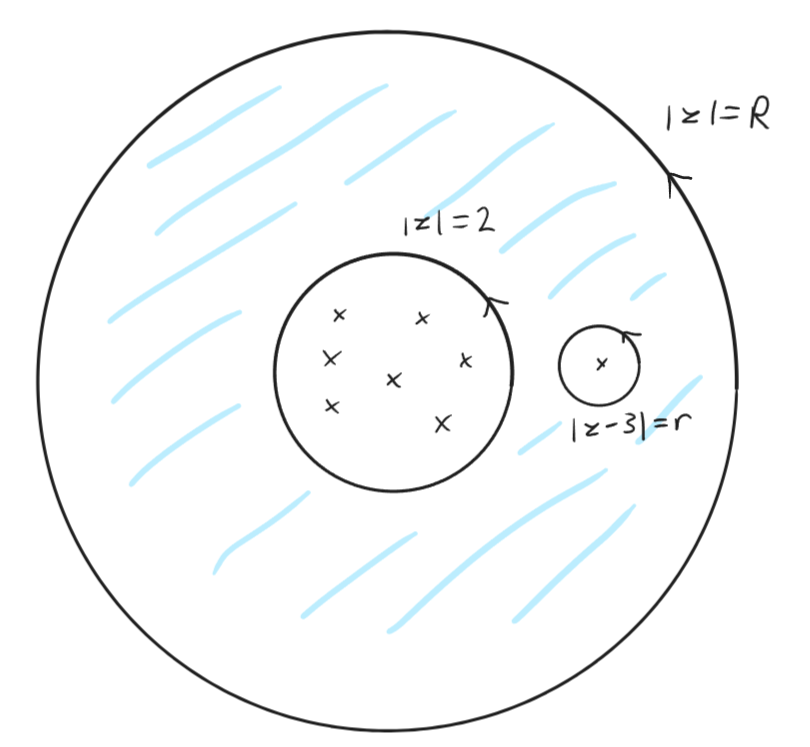
\includegraphics[width=0.5\textwidth]{Images/ComplexAnalysisPictures/DeformationOfPathEx.png}}
\begin{align*}
    &\text{ assume }|z^7+z+1|>0\text{ on }|z|>2\\
    &|z^7+z+1|\geq||z|^7-|z|-1|>|128-2-1|=125\\
    &\therefore\ \text{all 0s from $z^7+z+1$ inside region}\\
    &\lim_{R\to\infty}\int_{|z|=R}\frac{dz}{(z-3)(z^7+z+1)}=\int_{|z|=2}\frac{dz}{(z-3)(z^7+z+1)}+\lim_{r\to0}\int_{|z-3|=r}\frac{dz}{(z-3)(z^7+z+1)}\\
    &\int_{|z|=2}\frac{dz}{(z-3)(z^7+z+1)}=\lim_{R\to\infty}\int_{|z|=R}\frac{dz}{(z-3)(z^7+z+1)}-\lim_{r\to0}\int_{|z-3|=r}\frac{dz}{(z-3)(z^7+z+1)}\\
    &\lim_{r\to0}\int_{|z-3|=r}\frac{dz}{(z-3)(z^7+z+1)}=\lim_{r\to0}\int_{|z-3|=r}\frac{1}{z-3}f_1(3)dz\\
    &f_1(z)=\frac{1}{z^7+z+1}\Ra f_1(3)=\frac{1}{2191}\\
    &\lim_{r\to0}\int_{|z-3|=r}\frac{dz}{(z-3)(z^7+z+1)}=\frac{2\pi i}{2191}\\
    &\brvertical{\int_{|z|=R}\frac{dz}{(z-3)(z^7+z+1)}}\leq\max_{|z|=R}\brvertical{\frac{1}{(z-3)(z^7+z+1)}}2\pi R=\frac{2\pi R}{(R-3)(R^7-R-1)}\to0\\
    &\int_{|z|=2}\frac{dz}{(z-3)(z^7+z+1)}=-\frac{2\pi i}{2191}
\end{align*}
\textit{Extension of the Cauchy Integral Formula:}\\
If we have a pole (singularity) of order 2 at $z_0$ then we can extend the Cauchy Integral Formula
\begin{align*}
    &\int_C\frac{f(z)}{(z-z_0)}dz=2\pi if(z_0)\\
    &f(z_0)=\frac{1}{2\pi i}\int_C\frac{f(z)}{(z-z_0)}dz\\
    &f(z_0+\Delta z_0)=\frac{1}{2\pi i}\int_C\frac{f(z)}{z-(z_0+\Delta z_0)}dz\\
    &\frac{f(z_0+\Delta z_0)-f(z_0)}{\Delta z_0}=\frac{1}{2\pi i}\int_C\frac{f(z)}{\Delta z_0}\brround{\frac{1}{z-(z_0+\Delta z_0)}-\frac{1}{z-z_0}}dz\\
    &\frac{1}{z-(z_0+\Delta z_0)}-\frac{1}{z-z_0}=\frac{\Delta z_0}{(z-(z_0+\Delta z_0))(z-z_0)}\\
    &\frac{f(z_0+\Delta z_0)-f(z_0)}{\Delta z_0}=\frac{1}{2\pi i}\int_C\frac{f(z)}{\Delta z_0}\frac{\Delta z_0}{(z-(z_0+\Delta z_0))(z-z_0)}dz=\frac{1}{2\pi i}\int_C\frac{f(z)}{(z-(z_0+\Delta z_0))(z-z_0)}dz\\
    &\lim_{\Delta z_0\to0}\frac{f(z_0+\Delta z_0)-f(f_0)}{\Delta z_0}=\frac{1}{2\pi i}\lim_{\Delta z_0\to 0}\int_C\frac{f(z)}{(z-(z_0+\Delta z_0))(z-z_0)}dz\\
    &f'(z_0)=\frac{1}{2\pi i}\int_C\frac{f(z)}{(z-z_0)^2}dz
\end{align*}
Using the same technique we can generalize this to poles of order $m+1$
\[f^{(m)}(z_0)=\frac{m!}{2\pi i}\int_C\frac{f(z)}{(z-z_0)^{m+1}}dz\]
For $N$ poles, $z_1,\ldots,z_j$ of order $m_1+1,\ldots,m_j+1$ respectively, with $f(z)=\frac{1}{(z-z_j)^{m_j+1}}f_j(z)$ we get
\[\int_Cf(z)dz=2\pi i\sum_{j=1}^N\frac{f^{(m_j)}(z_j)}{m_j!}\]
Ex:
\begin{align*}
    &\int_{|z|=3}\frac{e^z}{(z^2+1)^2}dz\\
    &z=\pm i\\
    &f^{(m)}(z_0)=\frac{m!}{2\pi i}\int_C\frac{f(z)}{(z-z_0)^{m+1}}dz\\
    &z_1=i\\
    &f_1(z)=\frac{e^z}{(z+i)^2}\\
    &f_1'(z)=\frac{e^z}{(z+i)^2}-\frac{2e^z}{(z+i)^3}\\
    &f_1'(z_1)=\frac{e^i}{(2i)^2}-\frac{2e^{i}}{(2i)^3}=e^i\brround{\frac{1}{-4}-\frac{2}{-8i}}=\frac{e^i}{4}\brround{-1-i}\\
    &z_2=-i\\
    &f_2(z)=\frac{e^z}{(z-i)^2}\\
    &f_2'(z)=\frac{e^z}{(z-i)^2}-\frac{2e^z}{(z-i)^3}\\
    &f_2'(z_2)=\frac{e^{-i}}{(-2i)^2}-\frac{2e^{-i}}{(-2i)^3}=e^{-i}\brround{\frac{1}{-4}-\frac{2}{8i}}=\frac{e^{-i}}{4}\brround{-1+i}\\
    &\int_{|z|=3}\frac{e^z}{(z^2+1)^2}dz=2\pi if_1'(z_1)+2\pi if_2'(z_2)\\
    &=\frac{\pi}{2}\brround{e^i(1-i)+e^{-i}(-1-i)}\\
    &e^i=\cos(1)+i\sin(1)\\
    &e^{-i}=\cos(1)-i\sin(1)\\
    &I=\frac{\pi}{2}\brround{\cos(1)(1-i)+i\sin(1)(1-i)+\cos(1)(-1-i)-i\sin(1)(-1-i)}\\
    &=\frac{\pi}{2}\brround{-2i\cos(1)+2i\sin(1)}\\
    &=\pi i(\sin(1)-\cos(1))
\end{align*}
Ex2:
\begin{align*}
    &\int_{|z|=2}\frac{\cos(z)}{z^3(z-1)}dz\\
    &z_1=0,\ z_2=1\\
    &\int_{|z|=2}\frac{\cos(z)}{z^3(z-1)}dz=\frac{2\pi i}{2}f_1''(z_1)+2\pi if_2(z_2)\\
    &f_1(z)=\frac{\cos(z)}{z-1}\\
    &f_1'(z)=-\frac{\sin(z)}{z-1}-\frac{\cos(z)}{(z-1)^2}\\
    &f_1''(z)=-\frac{\cos(z)}{z-1}+\frac{2\sin(z)}{(z-1)^2}+\frac{2\cos(z)}{(z-1)^3}\\
    &f''_1(z_1)=-\frac{1}{-1}+0+\frac{2}{(-1)^3}=-1\\
    &f_2(z)=\frac{\cos(z)}{z^3}\\
    &f_z(z_2)=\frac{\cos(1)}{1}=\cos(1)\\
    &I=-\pi i+2\pi i\cos(1)
\end{align*}
Ex3:
\begin{align*}
    &\int_{|z|=2}\frac{z^2+1}{(z-1)^3}dz\\
    &z_0=1\\
    &\int_{|z|=2}\frac{z^2+1}{(z-1)^3}dz=\frac{2\pi i}{2}f''(z_0)\\
    &f(z)=z^2+1\\
    &f'(z)=2z\\
    &f''(z)=2=f''(z_0)\\
    &I=2\pi i
\end{align*}
Ex4:
\begin{align*}
    &\int_{|z-2|=1}\frac{\Log(z)}{(z^2-4)^2}dz\\
    &z=\pm 2\Ra z_0=2\\
    &\int_{|z-2|=1}\frac{\Log(z)}{(z^2-4)^2}dz=2\pi if'(z_0)\\
    &f(z)=\frac{\Log(z)}{(z+2)^2}\\
    &f'(z)=\frac{1/z}{(z+2)^2}-\frac{2\Log(z)}{(z+2)^3}\\
    &f'(2)=\frac{1/2}{4^2}-\frac{2\ln2}{4^3}=\frac{1}{32}-\frac{\ln2}{32}=\frac{1}{32}(1-\ln2)\\
    &I=\frac{\pi i}{16}(1-\ln2)
\end{align*}
Ex5:
\begin{align*}
    &\int_{|z|=2}\frac{e^{1/z}}{z^4+3z+1}dz\\
    &|z^4+3z+1|>0,\ |z|>2\\
    &|z^4+3z+1|\geq||z|^4-3|z|-1|>|16-6-1|=9\\
    &\int_{|z|=R}f(z)dz=\int_{|z|=2}f(z)dz\\
    &\brvertical{\int_{|z|=R}\frac{e^{1/z}}{z^4+3z+1}dz}\leq\max_{|z|=R}\brvertical{\frac{e^{1/z}}{z^4+3z+1}}2\pi R\\
    &\frac{1}{z}=\frac{\overline{z}}{|z|^2}\\
    &|e^{1/z}|=e^{\frac{x}{|z|^2}}\\
    &\max_{|z|=R}e^{\frac{x}{|z|^2}}=e^{\frac{R}{R^2}}=e^{\frac{1}{R}}\\
    &\brvertical{\int_{|z|=R}\frac{e^{1/z}}{z^4+3z+1}dz}\leq\frac{2\pi Re^{\frac{1}{R}}}{R^4-3R-1}\to0\text{ as }R\to\infty\\
    &I=0
\end{align*}
Ex6:
\begin{align*}
    &\int_{|z|=2}\frac{z}{(z-3)^2(z^3+z+1)}dz\\
    &|z^3+z+1|>0,\ |z|>2\\
    &|z^3+z+1|\geq||z|^3-|z|-1|>|8-2-1|=5\\
    &z_0=3\\
    &\int_{|z|=R} f(z)dz=\int_{|z|=2}f(z)dz+\int_{|z-3|=r}f(z)dz\\
    &\brvertical{\int_{|z|=R}\frac{z}{(z-3)^2(z^3+z+1)}dz}\leq\max_{|z|=R}\brvertical{\frac{z}{(z-3)^2(z^3+z+1)}}2\pi R=\frac{2\pi R^2}{(R-3)^2(R^3-R-1)}\to 0\\
    &\int_{|z-3|=r}\frac{z}{(z-3)^2(z^3+z+1)}dz=\int_{|z-3|=r}\frac{f_0(z)}{(z-3)^2}dz=2\pi if_0'(z_0)\\
    &f_0(z)=\frac{z}{z^3+z+1}\\
    &f_0'(z)=\frac{z^3+z+1-z(3z^2+1)}{(z^3+z+1)^2}\\
    &f_0'(z_0)=\frac{3^3+3+1-3(3^3+1)}{(3^3+3+1)^2}=-\frac{53}{961}\\
    &I=\frac{106}{961}\pi i
\end{align*}
We can also use this formula to compute some real integrals as well.\\
Ex:
\begin{align*}
    &\int_0^{2\pi}\frac{d\varphi}{3+\sin\varphi}\\
    &z=e^{i\varphi}\Ra dz=ie^{i\varphi}d\varphi=izd\varphi\Ra d\varphi=\frac{dz}{iz}\\
    &\sin\varphi=\frac{z-z^{-1}}{2i}\\
    &I=\int_{|z|=1}\frac{\frac{dz}{iz}}{3+\frac{z-z^{-1}}{2i}}=2\int_{|z|=1}\frac{dz}{6iz+z^2-1}\\
    &z_{1,2}=\frac{-6i\pm\sqrt{-36+4}}{2}=\frac{-6i\pm4\sqrt{2}i}{2}=-3i\pm2\sqrt{2}i\\
    &|z_1|=|-3i+2\sqrt{2}|\leq1\\
    &I=2\int_{|z-z_1|}\frac{dz}{(z-z_1)(z-z_2)}=\frac{4\pi i}{z_1-z_2}=\frac{4\pi i}{4\sqrt{2}i}=\frac{\pi}{\sqrt{2}}
\end{align*}
Ex2:
\begin{align*}
    &\int_0^\pi\frac{d\varphi}{2+\cos\varphi}\\
    &f(-\varphi)=\frac{1}{2+\cos(-\varphi)}=f(\varphi)\\
    &I=\frac{1}{2}\int_{-\pi}^\pi\frac{d\varphi}{2+\cos\varphi}\\
    &z=e^{i\varphi}\Ra dz=ie^{i\varphi}d\varphi=izd\varphi\Ra d\varphi=\frac{dz}{iz}\\
    &\cos\varphi=\frac{z+z^{-1}}{2}\\
    &I=\frac{1}{i}\int_{|z|=1}\frac{dz}{4z+z^2+1}\\
    &z_{1,2}=\frac{-4\pm\sqrt{16-4}}{2}=-2\pm\sqrt{3}\\
    &|z_1|=|-2+\sqrt{3}|\leq1\\
    &I=\frac{1}{i}\int_{|z-z_1|=r}\frac{dz}{(z-z_1)(z-z_2)}=\frac{1}{i}2\pi i\frac{1}{z_1-z_2}=\frac{2\pi}{2\sqrt{3}}=\frac{\pi}{\sqrt{3}}
\end{align*}
Ex3:
\begin{align*}
    &\int_0^\pi\frac{d\varphi}{(2+\cos\varphi)^2}=\frac{1}{2}\int_{-\pi}^\pi\frac{d\varphi}{(2+\cos\varphi)^2}\\
    &z=e^{i\varphi}\Ra dz=ie^{i\varphi}d\varphi=izd\varphi\Ra d\varphi=\frac{dz}{iz}\\
    &\cos\varphi=\frac{z+z^{-1}}{2}\\
    &I=\frac{2}{i}\int_{|z|=1}\frac{dz}{z(4+z+z^{-1})^2}=\frac{2}{i}\int_{|z|=1}\frac{zdz}{(4z+z^2+1)^2}\\
    &z_{1,2}=-2\pm\sqrt{3}\\
    &|z_1|=|-2+\sqrt{3}|\leq1\\
    &f_1(z)=\frac{z}{(z-z_2)^2}\\
    &f_1'(z)=\frac{(z-z_2)^2-2z(z-z_2)}{(z-z_2)^4}=\frac{z-z_2-2z}{(z-z_2)^3}\\
    &f_1'(z_1)=\frac{-z_1-z_2}{(z_1-z_2)^3}=\frac{4}{(2\sqrt{3})^3}=\frac{1}{2\sqrt{27}}\\
    &I=\frac{2}{i}2\pi if_1'(z_1)=\frac{2\pi}{3\sqrt{3}}
\end{align*}

\subsubsection{Applications of the Cauchy Integral Formula}
\textbf{Pointwise Estimate:}\\
We can estimate the maximum value of a point $z_0$ inside a closed path $C$.\\
Let us define a region enclosed by $|z-z_0|=R$ and start with the Cauchy Integral Formula
\begin{align*}
    &f^{(m)}(z_0)=\frac{m!}{2\pi i}\int_{|z-z_0|=R}\frac{f(z)}{(z-z_0)^{m+1}}dz\\
    &\brvertical{f^{(m)}(z_0)}=\frac{m!}{2\pi}\brvertical{\int_{|z-z_0|=R}\frac{f(z)}{(z-z_0)^{m+1}}dz}\leq\frac{m!}{2\pi}\max_{|z-z_0|=R}\brvertical{\frac{f(z)}{(z-z_0)^{m+1}}}2\pi R\\
    &\max_{|z-z_0|=R}|(z-z_0)^{m+1}|=R^{m+1}\\
    &\brvertical{f^{(m)}(z_0)}\leq\frac{m!}{2\pi}\max_{|z-z_0|=R}|f(z)|\frac{2\pi R}{R^{m+1}}\\
    &\brvertical{f^{(m)}(z_0)}\leq\frac{m!}{R^m}\max_{|z-z_0|=R}|f(z)|\\
\end{align*}
Ex: If $|f(z)|\leq 1$ on $|z|\leq 1$ estimate $f(0)$
\begin{align*}
    &|f^{(m)}(z_0)|\leq\frac{m!}{R^m}\max_{|z-z_0|=R}|f(z)|\\
    &z_0=0,\ R=1\\
    &|f''(0)|\leq \frac{2!}{1^2}\max_{|z|=1}|f(z)|\\
    &|f''(0)|\leq 2
\end{align*}
Ex2: If $|f(z)|\leq 1$ on $|z|\leq 1$ estimate $f(\tfrac{1}{2})$
\begin{align*}
    &|f^{(m)}(z_0)|\leq\frac{m!}{R^m}\max_{|z-z_0|=R}|f(z)|\\
    &z_0=\frac{1}{2},\ R=\frac{1}{2}\\
    &\max_{|z-\frac{1}{2}|=\frac{1}{2}}|f(z)|=\max_{|z-\frac{1}{2}|\leq\frac{1}{2}}|f(z)|=1\\
    &|f''(\tfrac{1}{2})|\leq\frac{2!}{(\tfrac{1}{2})^2}\max_{|z-\frac{1}{2}|=\frac{1}{2}}|f(z)|\\
    &|f''(\tfrac{1}{2})|\leq8
\end{align*}

\textbf{Liouville's Theorem:}\\
Recall that if $f(z)$ is entire then $f(z)$ is analytic in $C$. Liouville's Theorem states that if $f(z)$ is entire and bounded (i.e. $|f(z)|\leq M$) then $f(z)$ is constant.
\begin{proof}
Starting off from the pointwise estimate formula with $m=1$ we have
\[\brvertical{f'(z_0)}\leq\frac{1}{R}\max_{|z-z_0|=R}|f(z)|\]
Because $f(z)$ is bounded we have
\[\max_{|z-z_0|=R}|f(z)|=M\]
So we have
\[\brvertical{f'(z_0)}\leq\frac{M}{R}\]
Now because $f$ is entire we can take the limit as $R\to\infty$ and we get
\[|f'(z_0)|\leq 0\Ra f'(z)=0\]
So $f(z)$ is constant.
\end{proof}
We can also extend this to $m$th order derivatives in a more general manner.\\
Starting off from the pointwise estimate formula we got above we have
\[\brvertical{f^{(m)}(z_0)}\leq\frac{m!}{R^m}\max_{|z-z_0|=R}|f(z)|\]
Because $f(z)$ is bounded we have
\[\max_{|z-z_0|=R}|f(z)|=M\]
So we have
\[\brvertical{f^{(m)}(z_0)}\leq\frac{m!M}{R^m}\]
Now because $f$ is entire we can take the limit as $R\to\infty$ and we get
\[|f^{(m)}(z_0)|\leq 0\Ra f^{(m)}(z)=0\]
And so we can determine the degree of the polynomial $f(z)$ assuming we are provided information about which derivative is bounded.
Ex: Show that if $f(z)$ is entire and $|f(z)|\leq C(1+|z|)^4$ then $f(z)$ is a polynomial of at most degree 4.
\begin{align*}
    &|f^{(5)}(z_0)|\leq\frac{5!}{R^5}\max_{|z-z_0|=R}|f(z)|\\
    &|f(z)|\leq 2\max_{|z-z_0|=R}(1+|z|)^4\\
    &|f^{(5)}(z_0)|\leq\frac{240}{R^5}\max_{|z-z_0|=R}(1+|z|)^4\\
    &|z|\leq|z-z_0|+|z_0|\leq R+|z_0|\\
    &|f^{(5)}(z_0)|\leq\frac{240}{R^5}(1+R+|z_0|)^4\to0\text{ as }R\to\infty\\
    &|f^{(5)}(z_0)|=0\Ra f''''(z)=C_1\Ra f'''(z)=C_1z+C_2\Ra f''(z)=C_1z^2+C_2\\
    &\Ra f'(z)=C_1z^3+C_2z^2+C_3z+C_4\Ra f(z)=C_1z^4+C_2z^3+C_3z^2+C_4z+C_5\\
    &\mathrm{degree}(f(z))\leq 4
\end{align*}
We can also extend this further and say that for $f=u+iv$ if some linear combination of $u$ and $v$ is bounded then $f(z)$ is constant.\\
Ex: $u+v\geq 0$
\begin{align*}
    &f=u+iv\\
    &u+v\geq0\\
    &\Re((\alpha_1+i\alpha_2)(u+iv))=\alpha_1u-\alpha_2v\\
    &\alpha=1-i\\
    &g=e^{-\alpha f}\\
    &\text{$g$ is entire because $f$ is entire}\\
    &|g(z)|=|e^{\alpha f}|=|e^{-u-v}|\\
    &u+v\geq0\Ra e^{-u-v}\leq 1\\
    &|g(z)|\leq 1\\
    &|g'(z_0)|\leq\frac{1}{R}\max_{|z-z_0|=R}|g(z)|\to0\\
    &g'(z)=0\Ra g(z)\equiv C\\
    &\Ra f(z)\equiv C
\end{align*}

\textbf{Maximum Principle:}\\
If $f(z)$ is analytic in a region $D\cup\partial D$ then the maximum value on that region is equal to the maximum on the boundary
\[\max_{D\cup\partial D}|f(z)|=\max_{\partial D}|f(z)|\]
\begin{proof}
\[M=\max_{D\cup\partial D}|f(z)|=|f(z_0)|\]
for some $z_0\in D\cup\partial D$
Case 1: if $z_0\in\partial D$ then
\[M=|f(z_0)|\leq\max_{\partial D}|f(z)|\leq\max_{D\cup\partial D}|f(z)|=M\]
Case 2: $z_0\in D$
\begin{align*}
    &\brcurly{|z-z_0|\leq r}\subset D\\
    &f(z_0)=\frac{1}{2\pi i}\int_{|z-z_0|=r}\frac{f(z)}{z-z_0}dz\\
    &|f(z_0)|=M\leq\frac{1}{2\pi}\int_{|z-z_0|=r}\frac{|f(z)|}{|z-z_0|}dz=\frac{1}{2\pi}\int_0^{2\pi}|f(z_0+re^{i\theta})|d\theta\\
    &M=|f(z_0)|\leq\frac{1}{2\pi}\int_0^{2\pi}|f(z_0+re^{i\theta})|d\theta\\
    &\leq\frac{1}{2\pi}\int_0^{2\pi}\max_{D\cup\partial D}|f(z)|d\theta\\
    &\leq\frac{1}{2\pi}M\cdot 2\pi=M
\end{align*}
\end{proof}
We can also state the minimum principle which is very similar to the maximum principle.\\
Either 
\[\min_{D\cup\partial D}|f(z)|=\min_{\partial D}|f(z)|\]
or
\[\min_{D\cup\partial D}|f(z)|=0\]
Ex: Find the maximum and minimum values of $(z+1)^2e^{-z}$ on $|z|\leq 1$
\begin{align*}
    &\max_{|z|\leq1}|f(z)|=\max_{|z|=1}|f(z)|\\
    &z=e^{i\varphi}\\
    &|(z+1)^2e^{-z}|=|z+1|^2|e^{-z}|=((\cos \varphi+1)^2+\sin^2\varphi)e^{-\cos\varphi}=(2\cos\varphi+2)e^{-\cos\varphi}=h(\varphi)\\
    &h'(\varphi)=e^{-\cos\varphi}\brround{(2\cos\varphi+2)\sin\varphi-2\sin\varphi}=0\\
    &\sin\varphi\cos\varphi=0\Ra \varphi=\frac{n\pi}{2},\ n\in\Z\\
    &\cos\varphi=\brcurly{0,-1,1}\\
    &\mathrm{CPs}=\brcurly{2,4e^{-1},0}\\
    &\max_{|z|\leq1}|(z+1)^2e^{-z}|=2\\
    &\min_{|z|\leq1}|(z+1)^2e^{-z}|=0
\end{align*}
Ex2: Find the maximum and minimum values of $z^{100}+3z^{50}-1$ on $|z|\leq 1$
\begin{align*}
    &\max_{|z|\leq1}|f(z)|=\max_{|z|=1}|f(z)|\\
    &z=e^{i\varphi}\\
    &|z^{100}+3z^{50}-1|=|z^{50}||z^{50}+3-z^{-50}|=|e^{i50\varphi}+3-e^{-i50\varphi}|=|2i\sin(50\varphi)+3|=\sqrt{4\sin^2(50\varphi)+9}\\
    &\max_{\varphi}\sqrt{4\sin^2(50\varphi)+9}=\sqrt{13}
\end{align*}
\textbf{Argument Principle:}\\
This involves finding the zeros of a polynomial inside a given region (typically the positive real axis). Applications of this is used to determine the number of positive real roots of a polynomial which can be used to determine the stability of solutions to differential equations.\\
If $f(z)$ is analytic on $C$ and inside $C$ with $f(z)\neq0$ on $C$, $f(z)=0$ has finitely many roots inside $C$. Each root has multiplicity $n_j,\ j=1,\ldots,k$. Then,
\[\int_C\frac{f'(z)}{f(z)}dz=2\pi iN\]
where $N$ is the number of zeros of $f(z)$ inside $C$ (counting multiplicities) and is defined by
\[N=\sum_{j=1}^k n_j\]
\begin{align*}
    &C:\ z=z(t)\\
    &\int_C\frac{f'(z)}{f(z)}dz=\int_a^b\frac{f'(z(t))}{f(z(t))}z'(t)dt\\
    &w(t)=f(z(t))\Ra w'(t)=f'(z(t))z'(t)\\
    &\int_C\frac{f'(z)}{f(z)}dz=\int_a^b\frac{w'(t)}{w(t)}dt=\int_{w(a)}^{w(b)}\frac{dw}{w}=\int_{f(C)}\frac{dw}{w}=i\arg(w(t))\eval_{f(C)}\\
    &\int_C\frac{f'(z)}{f(z)}dz=i\arg(f(z))\eval_{f(C)}\\
    &\int_C\frac{f'(z)}{f(z)}dz=2\pi iN=i\arg(f(z))\eval_{f(C)}
\end{align*}
This leads us to the general form of the argument principle
\[N=\frac{1}{2\pi i}\int_C\frac{f'(z)}{f(z)}dz=\frac{\Arg(f(z))\eval_{f(C)}}{2\pi}\]
We can break this down into common applications.\\
\textbf{Rouche's Theorem:}\\
If $f(z)=g(z)+h(z)$ and $|h(z)|=|f(z)-g(z)|<|g(z)|$ on $C$ then the number of zeros in $f$ is the same as the number of zeros in $g$ ($N_f=N_g$).
\begin{proof}
\begin{align*}
    &f_\alpha(z)=g(z)+\alpha h(z),\ 0\leq\alpha\leq 1\\
    &f_0(z)=g(z),\ f_1(z)=f(z)\\
    &\frac{1}{2\pi i}\int_C\frac{f_\alpha'(z)}{f_\alpha(z)}dz=N(\alpha)=N_{f_\alpha}\\
    &\frac{1}{2\pi i}\int_C\frac{f_\alpha'(z)}{f_\alpha(z)}dz\text{ is continuous in }\alpha\\
    &N(\alpha)\text{ is continuous in }\alpha\\
    &\Ra N(\alpha)\text{ is constant in }\alpha\\
    &N(0)=N(1)\Ra N_g=N_f
\end{align*}
\end{proof}
Ex: Find the number of zeros of $z^5+2z^2-1$ in $|z|\leq1$
\begin{align*}
    &p(z)=z^5+2z^2+5z-1,\ |z|\leq 1\\
    &g(z)=5z\\
    &|g(z)|=5\\
    &|f(z)-g(z)|=|z^5+2z^2-1|\leq|z|^5+2|z|^2+1=4<5\\
    &N_f=N_g=1
\end{align*}
Ex2: Find the number of zeros of $8z^5+3z^4+4z^2-3$ in $|z|<1$
\begin{align*}
    &p(z)=8z^5+3z^4+4z^2-3,\ |z|<1\\
    &g(z)=8z^5\\
    &|g(z)|=8\\
    &|f(z)-g(z)|=|3z^4+4z^2-3|=|z|^2|3z^2-3z^{-2}+4|=|3z^2-3z^{-2}+4|\\
    &z=e^{i\varphi}\\
    &|f(z)-g(z)|=|3e^{2i\varphi}-3e^{-2i\varphi}+4|=|6i\sin(2\varphi)+4|=2\sqrt{9\sin^2(2\varphi)+4}\leq2\sqrt{13}<8\\
    &N_f=N_g=5
\end{align*}
Ex3: Find the number of zeros of $z^5+7z^2+2$ in $1\leq|z|\leq2$
\begin{align*}
    &p(z)=z^5+7z^2+2,\ 1\leq|z|\leq2\\
    &|z|=2:\\
    &g(z)=z^5\\
    &|g(z)|=32\\
    &|f(z)-g(z)|=|7z^2+2|\leq7|z|^2+2=30<32\\
    &N_f=N_g=5\\
    &|z|=1:\\
    &g(z)=7z^2\\
    &|g(z)|=7\\
    &|f(z)-g(z)|=|z^5+2|\leq|z|^5+2=3<7\\
    &N_f=N_g=2\\
    &\Ra N=5-2=3
\end{align*}
Ex4: Find the number of zeros of $z^2-4+3e^{-z}$ in $\Re(z)>0$
\begin{center}
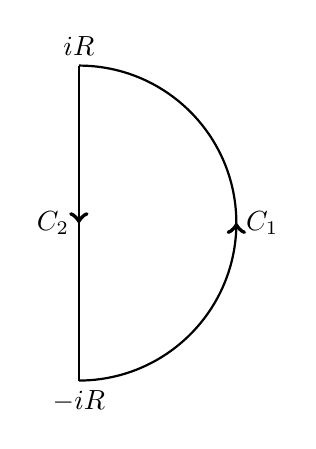
\begin{tikzpicture}
    % Half circle
    \draw[thick, decoration={markings,
        mark=at position 0.5 with {\arrow[line width=1.5pt]{>}}},
        postaction={decorate}]
    (0,-2) arc (-90:90:2);
    \draw[thick, decoration={markings,
        mark=at position 0.5 with {\arrow[line width=1.5pt]{>}}},
        postaction={decorate}]
    (0,2) -- (0,-2);
    
    % Labels
    \node[right] at (2,0) {$C_1$};
    \node[above] at (0,2) {$iR$};
    \node[below] at (0,-2) {$-iR$};
    \node[left] at (0,0) {$C_2$};
\end{tikzpicture}
\end{center}
\begin{align*}
    &f(z)=z^2-4+3e^{-z},\ \Re(z)>0\\
    &g(z)=z^2-4\\
    &h(z)=3e^{-z}\\
    &C=C_1\cup C_2\\
    &C_1:\ Re^{it},\ -\frac{\pi}{2}\leq t\leq \frac{\pi}{2}\\
    &C_2:\ iy,\ -R\leq y\leq R\\
    &C_1:\\
    &|h(z)|=3|e^{-z}|=3e^{-x}\leq 3\\
    &|g(z)|=|z^2-4|\geq|z|^2-4=R^2-4\\
    &R\to\infty:\ |g(z)|>|h(z)|\\
    &C_2:\\
    &|h(z)|=3e^{-x}=3\\
    &|g(z)|=|z^2-4|=|-y^2-4|=y^2+4\geq 4\\
    &|g(z)|>|h(z)|\\
    &g(z)=z^2-4=0\Ra z=\pm 2\Ra N_g=1\\
    &N_f=N_g=1
\end{align*}
Finding the number of zeros in the positive real part was a little complicated using Rouche's Theorem. Fortunately, there is a better method at solving this problem.\\
\textbf{Nyquist Criteria:}\\
From the argument principle we have
\[N_p=\frac{1}{2\pi}\arg(p(z))\eval_{p(C)}\]
Because we have $C$ broken into two parts, $C=C_1\cup C_2$, we get
\begin{align*}
    &\arg(p(z))\eval_{p(C)}=\arg(p)\eval_{p(C_1)}+\arg(p)\eval_{p(C_2)}\\
    &C_1:\ z=Re^{it},\ p(z)=a_nz^n+a_{n-1}z^{n-1}+\cdots=a_nRe^{int}+a_{n-1}R^{n-1}e^{i(n-1)t}+\cdots\\
    &-\pi\leq t\leq \pi\Ra \arg(p)\eval_{C_1}=n\pi
\end{align*}
For $C_2$, we can break it up into two paths for the positive and negative parts:
\begin{center}
    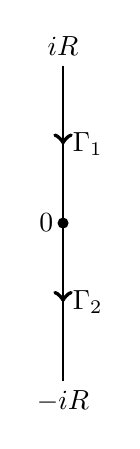
\begin{tikzpicture}
        % Half circle
        \fill (0,0) circle (2pt);
        \draw[thick, decoration={markings,
            mark=at position 0.5 with {\arrow[line width=1.5pt]{>}}},
            postaction={decorate}]
        (0,2) -- (0,0);
        \draw[thick, decoration={markings,
            mark=at position 0.5 with {\arrow[line width=1.5pt]{>}}},
            postaction={decorate}]
        (0,0) -- (0,-2);
        
        % Labels
        \node[right] at (0,1) {$\Gamma_1$};
        \node[above] at (0,2) {$iR$};
        \node[below] at (0,-2) {$-iR$};
        \node[right] at (0,-1) {$\Gamma_2$};
        \node[left] at (0,0) {$0$};
    \end{tikzpicture}
\end{center}
\begin{align*}
    &\arg(p)\eval_{p(\Gamma_1\cup\Gamma_2)}=\arg(p)\eval_{p(\Gamma_1)}+\arg(p)\eval_{\Gamma_2}\\
    &=\arg(p(i\infty))-\arg(p(0))+\arg(p(0))-\arg(p(-i\infty))\\
    &=\arg(p(i\infty))-\arg(p(-i\infty))\\
    &p(-iy)=\overline{p(iy)}\Ra p(-i\infty)=\overline{p(i\infty)}\\
    &\arg(p(-i\infty))=\arg(\overline{p(i\infty)})=-\arg(p(i\infty))\\
    &\arg(p)\eval_{p(\Gamma_1\cup\Gamma_2)}=2\arg(p)\eval_{p(\Gamma_1)}
\end{align*}
And so the number of zeros in the positive real part is
\[N=\frac{1}{2\pi}\brround{n\pi+2\arg(p)\eval_{p(\Gamma_1)}}\]
where $\Gamma_1:\ z=iy,\ 0<y<\infty$\\
Ex: Find the number of zeros of $z^3+2z^2+4$ in $\Re(z)>0$
\begin{align*}
    &p(z)=z^3+2z^2+4,\ \Re(z)>0\\
    &N=\frac{1}{2\pi}\brround{n\pi+2\arg(p)\eval_{p(\Gamma_1)}},\ n=3\\
    &\Gamma_1:\ z=iy,\ 0<y<\infty\\
    &p_R=-2y^2+4\\
    &p_I=-y^3\\
    &p_R=0\Ra -2y^2+4=0\Ra y^2=2\Ra y=\sqrt{2}
\end{align*}
\begin{tabular}{c|c|c}
    $y$ & $p_R$ & $p_I$\\
    \hline
    $\infty$ & $-\infty$ & $-\infty$\\
    $\sqrt{2}$ & 0 & $-2\sqrt{2}$\\
    0 & 4 & 0
\end{tabular}\\
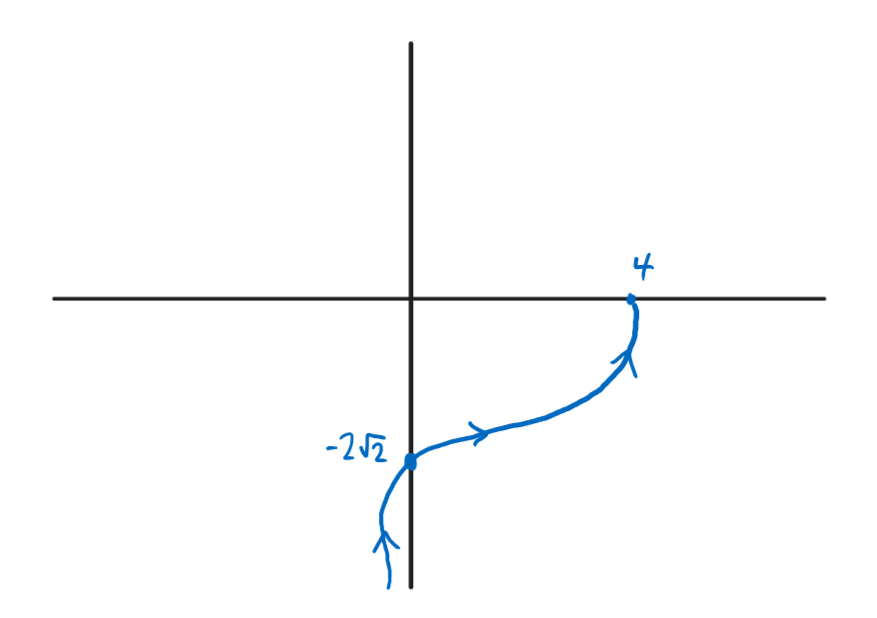
\includegraphics[scale=0.5]{Images/ComplexAnalysisPictures/Q5.png}
\begin{align*}
    &\arg(p)\eval_{p(\Gamma_1)}=\frac{\pi}{2}\\
    &N=\frac{1}{2\pi}\brround{3\pi+2\frac{\pi}{2}}=2
\end{align*}
Ex2: Find the number of zeros of $z^3+2z^2+4z+2$ in $\Re(z)>0$
\begin{align*}
    &p(z)=z^3+2z^2+4z+2\\
    &N=\frac{1}{2\pi}\brround{n\pi+2\arg(p)\eval_{p(\Gamma_1)}},\ n=3\\
    &\Gamma_1:\ z=iy,\ 0<y<\infty\\
    &p_R=-2y^2+2\\
    &p_I=-y^3+4y\\
    &p_R=0\Ra y^2=1\Ra y=1\\
    &p_I=0\Ra y(-y^2+4)=0\Ra y=0,\ y^2=4\Ra y=0,2
\end{align*}
\begin{tabular}{c|c|c}
    $y$ & $p_R$ & $p_I$\\
    \hline
    $\infty$ & $-\infty$ & $-\infty$\\
    2 & $-6$ & 0\\
    1 & 0 & 3\\
    0 & 2 & 0
\end{tabular}\\
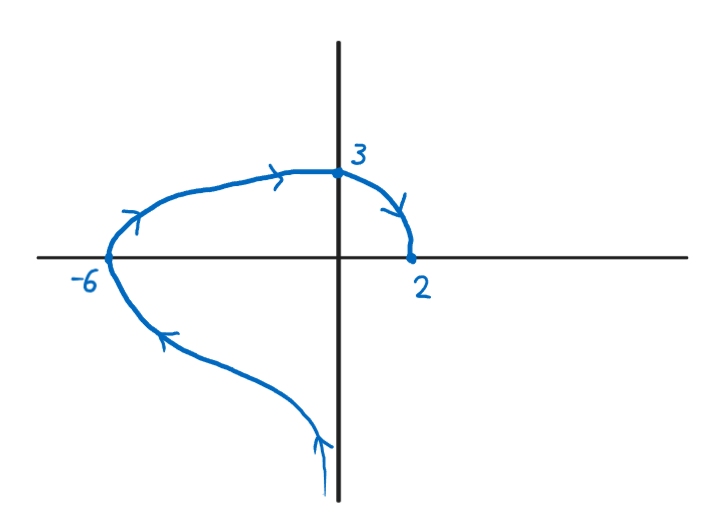
\includegraphics[scale=0.5]{Images/ComplexAnalysisPictures/Q6.png}
\begin{align*}
    &\arg(p)\eval_{p(\Gamma_1)}=-\frac{3\pi}{2}\\
    &N=\frac{1}{2\pi}\brround{3\pi+2\brround{-\frac{3\pi}{2}}}=0
\end{align*}
Ex3: Find the number of zeros of $z^3+z^2+4z+1$ in $\Re(z)>0$
\begin{align*}
    &p(z)=z^3+z^2+4z+1\\
    &N=\frac{1}{2\pi}\brround{n\pi+2\arg(p)\eval_{p(\Gamma_1)}},\ n=3\\
    &\Gamma_1:\ z=iy,\ 0<y<\infty\\
    &p_R=-y^2+1\\
    &p_I=-y^3+4y\\
    &p_R=0\Ra y=1\\
    &p_I=0\Ra y(-y^2+4)=0\Ra y=0,2
\end{align*}
\begin{tabular}{c|c|c}
    $y$ & $p_R$ & $p_I$\\
    \hline
    $\infty$ & $-\infty$ & $-\infty$\\
    2 & $-3$ & 0\\
    1 & 0 & 3\\
    0 & 1 & 0
\end{tabular}\\
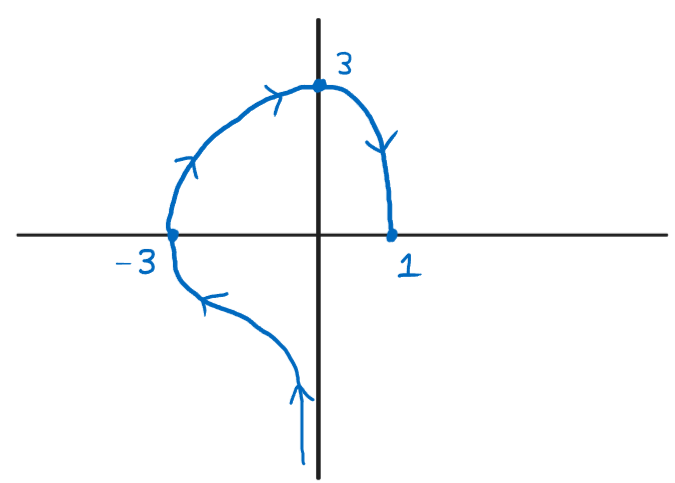
\includegraphics[scale=0.5]{Images/ComplexAnalysisPictures/Q7.png}
\begin{align*}
    &\arg(p)\eval_{p(\Gamma_1)}=-\frac{3\pi}{2}\\
    &N=\frac{1}{2\pi}\brround{3\pi+2\brround{-\frac{3\pi}{2}}}=0
\end{align*}

\subsubsection{Laurent Series}
Recall the Taylor series of a function is defined by
\[f(z)=\sum_{n=0}^\infty\frac{f^{(n)}(z_0)}{n!}(z-z_0)^n\]
The Taylor series will converge if $|z-z_0|<r$ where $r$ is the radius of convergence. The radius of convergence can be found to be
\[r=\min|z_0-\text{other singularities of }f(z)|\]
Some common Taylor series are
\begin{align*}
    &e^z=\sum_{n=0}^\infty\frac{z^n}{n!}\\
    &\sin z=\sum_{n=0}^\infty\frac{(-1)^nz^{2n+1}}{(2n+1)!}\\
    &\cos z=\sum_{n=0}^\infty\frac{(-1)^nz^{2n}}{(2n)!}\\
    &\frac{1}{1-z}=\sum_{n=0}^\infty z^n,\ |z|<1\\
    &\Log(1+z)=\sum_{n=1}^\infty\frac{(-1)^{n-1}z^n}{n},\ |z|<1
\end{align*}
The Laurent series is a generalization of the Taylor series that extends the Taylor series to negative exponentials in the series. If we compare the two we get,\\
\textit{Taylor Series:}\\
$f$ is analytic in $|z-z_0|<r$
\[f(z)=\sum_{n=0}^\infty a_n(z-z_0)^n\]
\[a_n=\frac{f^{(n)}(z_0)}{n!}=\frac{1}{2\pi i}\int_{|z-z_0|=r}\frac{f(\eta)}{(\eta-z_0)^{n+1}}d\eta\]
\textit{Laurent Series:}\\
$f$ is analytic in $r_1<|z-z_0|<r_2$
\[f(z)=\sum_{n=-\infty}^\infty a_n(z-z_0)^n\]
\[a_n=\frac{1}{2\pi i}\int_{|z-z_0|=r}\frac{f(\eta)}{(\eta-z_0)^{n+1}}d\eta\]
Ex: Find the Laurent series of $f(z)=\frac{z}{(z+1)(z-2)}$ in each of $|z|<1$, $1<|z|<2$, and $|z|>2$
\begin{align*}
    &f(z)=\frac{z}{(z+1)(z-2)}\\
    &f(z)=\frac{A}{z+1}+\frac{B}{z-2}\\
    &A+B=1\\
    &-2A+B=0\Ra 2A=B\\
    &3A=1\Ra A=\frac{1}{3}\Ra B=\frac{2}{3}\\
    &f(z)=\frac{1}{3}\brround{\frac{1}{z+1}+\frac{2}{z-2}}
\end{align*}
\begin{align*}
    &|z|<1\\
    &\frac{1}{1+z}=1-z+z^2-z^3+\cdots=\sum_{n=0}^\infty(-1)^nz^n\\
    &\frac{1}{1-z}=1+z+z^2+z^3+\cdots=\sum_{n=0}^\infty z^n\\
    &f(z)=\frac{1}{3}\brround{\frac{1}{z+1}-\frac{1}{1-\frac{z}{2}}}\\
    &f(z)=\frac{1}{3}\sum_{n=0}^\infty\brround{(-1)^n-\frac{1}{2^n}}z^n
\end{align*}
\begin{align*}
    &|z|>2\\
    &\frac{1}{z+1}=\frac{1}{z}\frac{1}{1-(-\frac{1}{z})}=\frac{1}{z}\sum_{n=0}^\infty\bfrac{-1}{z}^n\\
    &\frac{1}{z-2}=\frac{1}{z}\frac{1}{1-\frac{2}{z}}=\frac{1}{z}\sum_{n=0}^\infty\bfrac{2}{z}^n\\
    &f(z)=\frac{1}{3}\sum_{n=0}^\infty\brround{(-1)^n+2^{n+1}}\frac{1}{z^{n+1}}
\end{align*}
\begin{align*}
    &1<|z|<2\\
    &\frac{1}{z+1}=\frac{1}{z}\frac{1}{1-(-\frac{1}{z})}=\frac{1}{z}\sum_{n=0}^\infty\bfrac{-1}{z}^n\\
    &\frac{1}{z-2}=-\frac{1}{2}\frac{1}{1-\frac{z}{2}}=-\frac{1}{2}\sum_{n=0}^\infty\bfrac{z}{2}^n\\
    &f(z)=\frac{1}{3}\sum_{n=0}^\infty\brround{\frac{(-1)^n}{z^{n+1}}-\frac{z^n}{2^{n}}}
\end{align*}
Big O Notation:\\
When $n$ gets very large then $\mathcal{O}(n)$ determines how fast the function grows.
\[\mathcal{O}(n)\Leftrightarrow |\mathcal{O}(n)|\leq C|n|\]
When $n$ gets very small then $o(n)$ determines how fast the function shrinks.
\[o(n)\Leftrightarrow \frac{o(n)}{n}\to 0\text{ as }n\to 0\]
Ex2: Find the first few terms of the Laurent series for $f(z)=\frac{z}{\Log z},\ |z-1|<1$
\begin{align*}
    &f(z)=\frac{z}{\Log z},\ |z-1|<1\\
    &\Log(z)=\Log(z-1+1)\\
    &w=z-1\\
    &\Log(z)=\Log(w+1)=w-\frac{w^2}{2}+\frac{w^3}{3}-\mathcal{O}(w^4)=w\brround{1-\frac{w}{2}+\frac{w^2}{3}-\mathcal{O}(w^3)}\\
    &\frac{1}{\Log(z)}=\frac{1}{w}\frac{1}{1-\frac{w}{2}+\frac{w^2}{3}-\mathcal{O}(w^3)}\\
    &w_1=\frac{w}{2}-\frac{w^2}{3}+\mathcal{O}(w^3)\\
    &\frac{1}{1-w_1}=1+w_1+w_1^2+\mathcal{O}(w_1^3)\\
    &\frac{1}{1-w_1}=1+\frac{w}{2}-\frac{w^2}{3}+\frac{w^2}{4}+\mathcal{O}(w^3)=1+\frac{w}{2}-\frac{w^2}{12}+\mathcal{O}(w^3)\\
    &\frac{1}{\Log(z)}=\frac{1}{w}+\frac{1}{2}-\frac{w}{12}+\mathcal{O}(w^2)\\
    &\frac{z}{\Log(z)}=(w+1)\brround{\frac{1}{w}+\frac{1}{2}-\frac{w}{12}+\mathcal{O}(w^2)}\\
    &\frac{z}{\Log(z)}=\frac{1}{w}+\frac{1}{2}-\frac{w}{12}+1+\frac{w}{2}+\mathcal{O}(w^2)=\frac{1}{w}+\frac{3}{2}+\frac{5}{12}w+\mathcal{O}(w^2)\\
    &\frac{z}{\Log(z)}=\frac{1}{z-1}+\frac{3}{2}+\frac{5}{12}(z-1)+\mathcal{O}((z-1)^2)
\end{align*}
Ex3: Find the Laurent series for $f(z)=\frac{1}{z(z-2)},\ 1<|z+1|<3$
\begin{align*}
    &f(z)=\frac{1}{z(z-2)},\ 1<|z+1|<3\\
    &f(z)=\frac{1}{(z+1-1)(z+1-3)}\\
    &w=z+1\\
    &f(z)=\frac{1}{(w-1)(w-3)}\\
    &=\frac{A}{w-1}+\frac{B}{w-3}\\
    &A+B=0\Ra A=-B\\
    &-3A-B=1\Ra 3B-B=1\Ra 2B=1\Ra B=\frac{1}{2}\Ra A=-\frac{1}{2}\\
    &f(z)=\frac{1}{2}\brround{\frac{1}{w-3}-\frac{1}{w-1}}\\
    &=\frac{1}{2}\brround{-\frac{1}{3}\frac{1}{1-\frac{w}{3}}-\frac{1}{w}\frac{1}{1-\frac{1}{w}}}\\
    &=-\frac{1}{2}\brround{\frac{1}{3}\sum_{n=0}^\infty\bfrac{w}{3}^n+\frac{1}{w}\sum_{n=0}^\infty\bfrac{1}{w}^n}\\
    &=-\frac{1}{6}-\frac{1}{2}\sum_{n=1}^\infty\brround{\frac{w^n}{3^{n+1}}+\frac{1}{w^n}}\\
    &f(z)=-\frac{1}{6}-\frac{1}{2}\sum_{n=1}^\infty\brround{\frac{(z+1)^n}{3^{n+1}}+\frac{1}{(z+1)^n}}
\end{align*}
Ex4: Find the Laurent series for $f(z)=\frac{1}{z^2+1},\ |z-i|>2$
\begin{align*}
    &f(z)=\frac{z}{z^2+1},\ |z-i|>2\\
    &z^2+1=(z+i)(z-i)=(z-i+2i)(z-i)\\
    &f(z)=\frac{z-i+i}{(z-i)(z-i+2i)}\\
    &w=z-i\\
    &f(z)=\frac{w+i}{w(w+2i)}=\frac{1}{w+2i}+\frac{i}{w}\frac{1}{w+2i}\\
    &\frac{1}{w+2i}=\frac{1}{w}\frac{1}{1+\frac{2i}{w}}=\frac{1}{w}\sum_{n=0}^\infty\bfrac{-2i}{w}^n\\
    &f(z)=\sum_{n=0}^\infty\brround{\frac{(-2i)^n}{w^{n+1}}+\frac{(-1)^n2^ni^{n+1}}{w^{n+2}}}\\
    &=\frac{1}{w}+\sum_{n=0}^\infty\brround{\frac{(-2i)^{n+1}}{w^{n+2}}+\frac{(-1)^n2^ni^{n+1}}{w^{n+2}}}=\frac{1}{w}+\sum_{n=0}^\infty\frac{2^ni^{n+1}}{w^{n+2}}(-2+1)\\
    &f(z)=\frac{1}{z-i}-\sum_{n=0}^\infty\frac{(-2)^ni^{n+1}}{(z-i)^{n+2}}
\end{align*}
Ex5: Find the Laurent series for $\sqrt{z}$ about $z_0=1$
\begin{align*}
    &\sqrt{z},\ z_0=1\\
    &w=z-z_0=z-1\\
    &\sqrt{z}=\sqrt{z+1-1}=\sqrt{w+1}\\
    &(1+w)^r=\sum_{n=0}^\infty\combm{r}{n}w^n\\
    &\sqrt{w+1}=\sum_{n=0}^\infty\combm{\frac{1}{2}}{n}w^n\\
    &\sqrt{z}=\sum_{n=0}^\infty\combm{\frac{1}{2}}{n}(z-1)^n\approx 1+\frac{1}{2}(z-1)+\frac{\frac{1}{2}(\frac{1}{2}-1)}{2!}(z-1)^2+\frac{\frac{1}{2}(\frac{1}{2}-1)(\frac{1}{2}-2)}{3!}(z-1)^3+\cdots
\end{align*}
Ex6: Find the Laurent series for $f(z)=\frac{e^z}{1-z}$ about $z_0=0$
\begin{align*}
    &\frac{e^z}{1-z},\ z_0=0\\
    &e^z=\sum_{n=0}^\infty\frac{z^n}{n!}\\
    &\frac{1}{1-z}=\sum_{n=0}^\infty z^n\\
    &f(z)=\sum_{m=0}^\infty z^m\sum_{n=0}^\infty\frac{z^n}{n!}=(1+z+z^2+\mathcal{O}(z^3))\brround{1+z+\frac{z^2}{2!}+\mathcal{O}(z^3)}\\
    &f(z)=\sum_{n=0}^\infty\brround{\sum_{m=0}^n\frac{1}{m!}}z^n\approx1+\brround{1+\frac{1}{1!}}z+\brround{1+\frac{1}{1!}+\frac{1}{2!}}z^2+\cdots
\end{align*}
\subsubsection{Cauchy Residue Theorem}
Classification of Singularities:\\
For a Laurent series of $f(z)$ in $r_1<|z-z_0|<r_2$ with $f(z)=a_0+a_1(z-z_0)+\cdots+a_n(z-z_0)^n+a_{-1}(z-z_0)^{-1}+\cdots+a_{-n}(z-z_0)^{-n}$ we can classify singularities as follows:
\begin{itemize}
    \item If $a_{-1}=a_{-2}=\cdots=a_{-n}=0$ (all negative terms) then $z_0$ is a removable singularity
    \item If $a_{-n}=0,\ n\geq m+1$ (finite negative terms) then $z_0$ is a pole of order $m$\\
    If $m=1$ then it is called a simple pole
    \item If $a_{-n}\neq0$ for all $n$ then $z_0$ is an essential singularity
\end{itemize}
The \textit{residue} of $f(z)$ at $z_0$ is defined to be the $a_{-1}$ coefficient of the Laurent series of $f(z)$ about $z_0$.
\[a_{-1}=\Res(f;z_0)\]
Ex: Find the residue of $f(z)=\frac{1+2z^2}{z^5+z^3}$ about $z_0=0$
\begin{align*}
    &f(z)=\frac{1+2z^2}{z^5+z^3},\ z_0=0\\
    &f(z)=\frac{1}{z^3}\brround{1+2z^2}\brround{z^2+1}^{-1}\\
    &(z^2+1)^{-1}=1-z^2+\frac{-1(-1-1)}{2}z^4+\bigO(z^6)\\
    &f(z)=\frac{1}{z^3}\brround{1+2z^2}\brround{1-z^2+z^4+\bigO(z^6)}=\frac{1}{z^3}\brround{1-z^2+z^4+2z^2-2z^4+\bigO(z^6)}\\
    &f(z)=\frac{1}{z^3}+\frac{1}{z}-z+\bigO(z^3)\\
    &\Res\brround{f(z);0}=1
\end{align*}
